%%%%%%%%%%%%%%%%%%%%%%%%%%%%%%%%%%%%%%%%%
% Luca Maurelli CV
%%%%%%%%%%%%%%%%%%%%%%%%%%%%%%%%%%%%%%%%%

%----------------------------------------------------------------------------------------
%	PACKAGES AND OTHER DOCUMENT CONFIGURATIONS
%----------------------------------------------------------------------------------------

\documentclass[10pt]{article}

%\usepackage{showframe}
\usepackage[a4paper,
			includeheadfoot,
			top = 1cm,
			bottom = 0cm,
			left = 1cm,
			right = 1cm]{geometry}

\usepackage{fancyhdr}

% interpreters
\usepackage[utf8]{inputenc}
\usepackage[T1]{fontenc}

% language
\usepackage[english]{babel}
\usepackage{csquotes}

% font
\usepackage{libertine}
\usepackage{courier}
\usepackage{fontawesome5}

% Paragraph indentation: empty line rather than an indent
\usepackage[parfill]{parskip}

\usepackage{booktabs}
\usepackage{graphicx}

\usepackage{enumitem}
\setlist[enumerate,1]{label=$\vcenter{\hbox{\tiny$\bullet$}}$,leftmargin=*}
\setlist[enumerate,2]{label=--,leftmargin=*}

\usepackage[dvipsnames]{xcolor}
\usepackage[allbordercolors = red,
			colorlinks = true,
            linkcolor = BrickRed,
            urlcolor  = BrickRed,
            citecolor = BrickRed,
            anchorcolor = BrickRed]{hyperref}

\usepackage{cleveref}

\fancyhead[L]{\textit{Luca Maurelli's Curriculum Vitae}}
\fancyhead[C]{\textsc{Data Scientist | Data Engineer}}
\fancyhead[R]{\thepage}
\fancyfoot[L]{}
\fancyfoot[C]{}
\fancyfoot[R]{}
\renewcommand{\headrulewidth}{0pt}
\renewcommand{\footrulewidth}{0pt}


\newcommand{\cvsection}[1]{\section*{\centering\normalsize\uppercase{#1}}\vspace{-16pt}\rule{\linewidth}{0.2pt}\vspace{6pt}}

% debug
% \usepackage{showframe}

\begin{document}
% empty header and footer
% https://tex.stackexchange.com/questions/194423/page-style-plain-vs-empty
\pagestyle{empty}

%----------------------------------------------------------------------------------------
%	TITLE PAGE
%----------------------------------------------------------------------------------------
\centering
{\huge\textsc{Luca~Maurelli's~Curriculum~Vitae}\par}
{\textsc{Data Scientist | Data Engineer}\par}
%{\textsc{Updated:~}\today\par}
\raggedright
%\vspace{1cm}

%----------------------------------------------------------------------------------------
%   PERSONAL DATA
%----------------------------------------------------------------------------------------
\cvsection{personal data}

\noindent
\begin{minipage}[t]{.6\linewidth}
	\raggedright
	\begin{tabular}{@{}ll@{}}
	name \& surname:&Luca Maurelli\\
	sex \& pronouns:&\faIcon{male} Male, \faIcon{mars-double} He\textbackslash Him\\
	birthdate \& birthplace:&June 30, 1993 in Milan, Italy\\
	contacts:&\faIcon{phone} \href{tel:+393408192088}{(+39)~340~8192088} \faIcon{envelope} \href{mailto:lucamaurelli93@gmail.com}{lucamaurelli93@gmail.com}\\
	% phone: & \href{tel:+393408192088}{(+39)~340~8192088} \\
	%e-mail: & \href{mailto:luca.maurelli@unibg.it}{luca.maurelli@unibg.it} \\
	% e-mail: & \href{mailto:lucamaurelli93@gmail.com}{lucamaurelli93@gmail.com} \\
	location:&\faIcon{map-marker-alt} \href{https://goo.gl/maps/ir6c5EaAzBuvGFTb6}{Treviglio~(BG),~24047,~Italy}\\
	languages:&\faIcon{language} Italian, English (spoken B2, written C1)\\
	driving license:&\faIcon{car} B (cars) 
	\end{tabular}
\end{minipage}
\hfill
\begin{minipage}{.3\linewidth}
	\raggedleft
	%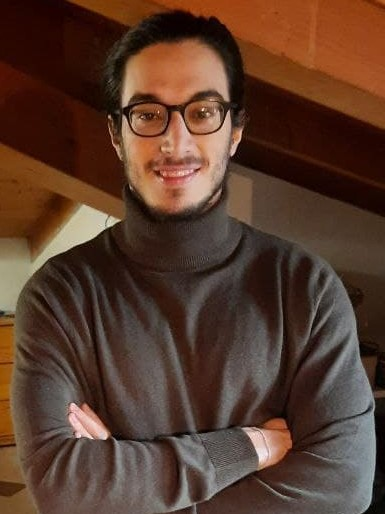
\includegraphics[width=3cm]{face.jpg}
\end{minipage}

% \begin{minipage}[t]{.5\linewidth}
% 	\raggedleft
% 	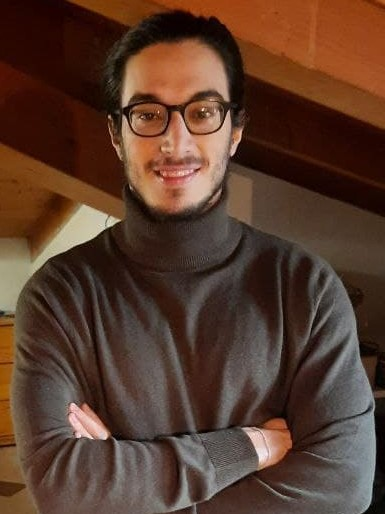
\includegraphics[height=3cm]{face.jpg}
% \end{minipage}

% \begin{tabular}[t]{@{}ll@{}}
% 	name \& surname:&Luca Maurelli\\
% 	sex \& pronouns:&\faIcon{male} Male, \faIcon{mars-double} He\textbackslash Him\\
% 	birthdate \& birthplace:&June 30, 1993 in Milan, Italy\\
% 	contacts:&\faIcon{phone} \href{tel:+393408192088}{(+39)~340~8192088} \faIcon{envelope} \href{mailto:lucamaurelli93@gmail.com}{lucamaurelli93@gmail.com}\\
% 	location:&\faIcon{map-marker-alt} \href{https://goo.gl/maps/ir6c5EaAzBuvGFTb6}{Treviglio~(BG),~24047,~Italy}\\
% 	languages:&\faIcon{language} Italian, English (spoken B2, written C1)\\
% 	driving license:&\faIcon{car} B (cars) 
% \end{tabular}
% \begin{minipage}[c]{3cm}
% 	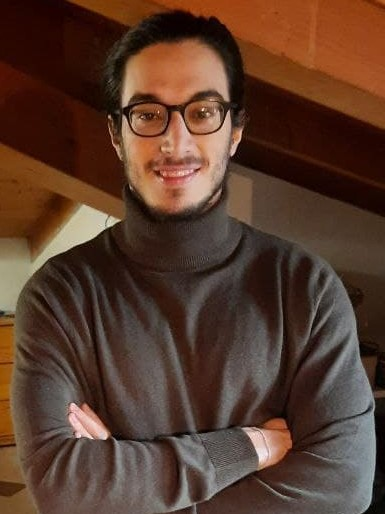
\includegraphics[width=3cm]{face.jpg}
% \end{minipage}

%----------------------------------------------------------------------------------------
%	WORK EXPERIENCES SECTION
%----------------------------------------------------------------------------------------
\cvsection{Job Experience}

\noindent
\begin{minipage}[t]{.8\textwidth}
	\textbf{Ph.D. Student} at the \href{https://disa.unibg.it/}{Department of Engineering and Applied Sciences}
	\begin{enumerate}
		\item Theoretical research on the design and estimation of a data-driven direct filter in a stochastic framework formulation and comparison with standard filtering solutions\\
		({\scriptsize \textbf{tools:} \href{https://www.mathworks.com/products/matlab.html}{MATLAB}, \href{https://yalmip.github.io/}{YALMIP} \& \href{https://www.mosek.com/}{Mosek}\textbackslash \href{https://www.gurobi.com/}{Gurobi} for SDP})

		\item Project \href{https://www.smart4cpps.it/}{SMART4CPPS}, funded by Regione Lombardia, led by 4 OdR and 10 local companies.
		\begin{enumerate}
			\item Management activity of Pilot 1 and Pilot 4
			\item Technical activity of Pilot 1: Design of a health monitoring system for electromechanical actuators ({\small University of Bergamo, Camozzi})
			\item Technical activity of Pilot 4: Machine learning algorithms for the zero-defect end-of-line tuning of medium-voltage switches ({\small University of Bergamo, Cosberg, ABB, CNR})\\
			({\scriptsize \textbf{tools:} MATLAB})
		\end{enumerate}
		\item Publication of international journal papers and patents regarding academic and industrial results, see items from \ref{c2020} to \ref{p2022}.\\
		({\scriptsize \textbf{tools:} \href{https://www.latex-project.org/}{LaTeX}, \href{https://www.lyx.org/LyX}{LyX}, PowerPoint, \href{https://code.visualstudio.com/}{VS Code}})
	\end{enumerate}
\end{minipage}% note the use of "%"
\hfill\vrule\hfill
\begin{minipage}[t]{.16\textwidth}
	\raggedleft
	Oct 2019 – Current\\
	{\small University of Bergamo}
\end{minipage}

%----------------------------------------------------------------------------------------
\vspace{6pt} % Gap between titles
%----------------------------------------------------------------------------------------

\noindent
\begin{minipage}[t]{.8\textwidth}
	\raggedright
	\textbf{Research Assistant} at the \href{https://digip.unibg.it/}{Department of Management, Information and Production Engineering}
	\begin{enumerate}
		\item Project CRYOABLATION:
		\begin{enumerate}
			\item Identification of a model and validation of the structure for the study of temperature dynamics in the cryoablation process for atrial fibrillation therapy ({\small Dipartimento di Cardiologia, Ospedale di Seriate})\\
			({\scriptsize \textbf{tools:} \href{https://www.mathworks.com/products/matlab.html}{MATLAB}})
		\end{enumerate}
		\item Project SP@RK-4.0-I.E.S.:
		\begin{enumerate}
			\item Supported design and implementation of a prototype for the acquisition of experimental data in the development of a predictive maintenance system through the analysis of acceleration signals for the fault diagnosis of rotating components (bearings) in high performance work-centers ({\small Mandelli})\\
			({\scriptsize \textbf{tools:} \href{https://www.mathworks.com/products/matlab.html}{MATLAB}, \href{https://www.ni.com/it-it/shop/data-acquisition.html}{NI C-Daq}, \href{https://www.ni.com/it-it/shop/labview.html}{LabView}})
		\end{enumerate}
  \end{enumerate}
\end{minipage}% note the use of "%"
\hfill\vrule\hfill
\begin{minipage}[t]{.16\textwidth}
	\raggedleft
	May 2018 – Sep 2019\\
	{\small University of Bergamo}
\end{minipage}

% OLD

% \noindent
% \begin{minipage}[t]{.8\textwidth}
% 	\raggedright
% 	\textbf{Research Assistant} at the \href{https://digip.unibg.it/}{Department of Management, Information and Production Engineering}
% 	\begin{enumerate}
% 		\item Project SMART4CPPS, funded by Regione Lombardia, led by 4 OdR and 10 local companies.
% 		\begin{enumerate}
% 			\item Management activity of Pilot 1 and Pilot 4
% 			\item Technical activity of Pilot 1: Design of a health monitoring system for electromechanical actuators (University of Bergamo, Camozzi)
% 			\item Technical activity of Pilot 4: Machine learning algorithms for the zero-defect end-of-line tuning of medium-voltage switches (University of Bergamo, Cosberg, ABB, CNR)
% 		\end{enumerate}
% 		\item Project CRYOABLATION:
% 		\begin{enumerate}
% 			\item Model identification of the temperature dynamics in \textit{cryoblation} for atrial fibrillation therapy (Dipartimento di Cardiologia, Ospedale di Seriate)
% 		\end{enumerate}
% 		\item Project SP@RK-4.0-I.E.S.:
% 		\begin{enumerate}
% 			\item Data analysis and development of a health monitoring and predictive maintenance system in high performance workcenters (Mandelli spa)
% 		\end{enumerate}
% 		\item Project SMI-PREDICTIVE MAINTENANCE:
% 		\begin{enumerate}
% 			\item Design of a predictive maintenance system for beverage packaging machines using accelerometers (SMI Group)
% 		\end{enumerate}
%   \end{enumerate}
% \end{minipage}% note the use of "%"
% \hfill\vrule\hfill
% \begin{minipage}[t]{.16\textwidth}
% 	\raggedleft
% 	May 2018 – Sep 2019\\
% 	{\small University of Bergamo}
% \end{minipage}

%----------------------------------------------------------------------------------------
\vspace{6pt} % Gap between titles
%----------------------------------------------------------------------------------------

\noindent
\begin{minipage}[t]{.8\textwidth}
	\raggedright
	\textbf{Software Engineer} at \href{https://www.intellimech.it/}{Consortium Intellimech} (Intership during Master's thesis)
	\begin{enumerate}
		\item Project KNOWLEDGIZE, funded by Regione Lombardia, led by Consortium Intellimech, with 2 OdR and 3 local companies.
		  \begin{enumerate}
			\item Development of a Django-based web platform for corporate knowledge management by searching for similar tags on content using ML algorithms related to natural language processing through Google cloud services ({\small University of Bergamo, University of Brescia, Cosberg, Elettrocablaggi, Ronzoni})\\
			({\scriptsize \textbf{tools:} \href{https://www.djangoproject.com/}{Django}, \href{https://www.python.org/}{Python}, \href{https://github.com/RaRe-Technologies/gensim}{Gensim} word2vec Skip-Gram model})
		\end{enumerate}
		\item Supported development of software applications:
		  \begin{enumerate}
			\item Push-bottom panel for testing procedures on a PLC in C\#
			\item Development of a monitoring system through an MQTT publisher-subscriber infrastructure between gateway and industrial nodes with support to different communication protocols (MQTT, MTCONNECT, UPC-UA and MODbus) in Python
		\end{enumerate}
  \end{enumerate}
\end{minipage}% note the use of "%"
\hfill\vrule\hfill
\begin{minipage}[t]{.16\textwidth}
	\raggedleft
	Oct 2017 – Apr 2018
\end{minipage}

% OLD

% \noindent
% \begin{minipage}[t]{.8\textwidth}
% 	\raggedright
% 	\textbf{Software Engineer} at \href{https://www.intellimech.it/}{Consortium Intellimech} (Intership during Master's thesis)
% 	\begin{enumerate}
% 		\item Project KNOWLEDGIZE, funded by Regione Lombardia, led by Consortium Intellimech, with 2 OdR and 3 local companies.
% 		  \begin{enumerate}
% 			\item Development of a Knowledge Management Web Platform with an Innovative ML Algorithm based on Tag Searching using Django and Google Services (University of Bergamo, University of Brescia, Cosberg, Elettrocablaggi, Vin Service)
% 		\end{enumerate}
% 		\item Development of software applications:
% 		  \begin{enumerate}
% 			\item Push-bottom panel for testing procedures on PLC in C\#
% 			\item Monitoring system using industrial communicating protocols MQTT, MTCONNECT, UPC-UA and MODbus in Python
% 		\end{enumerate}
%   \end{enumerate}
% \end{minipage}% note the use of "%"
% \hfill\vrule\hfill
% \begin{minipage}[t]{.16\textwidth}
% 	\raggedleft
% 	Oct 2017 – Apr 2018%\\
% 	%\href{https://www.linkedin.com/company/kilometro-rosso/}{Kilometro Rosso}
% 	%{\small Kilometro Rosso}
% \end{minipage}

%----------------------------------------------------------------------------------------
%	NEW PAGE
%----------------------------------------------------------------------------------------
\clearpage
\pagestyle{fancy}

%----------------------------------------------------------------------------------------
%	EDUCATION SECTION
%----------------------------------------------------------------------------------------

\cvsection{education}
\textbf{Master's degree in Computer Science}, University of Bergamo, Italy \hfill 110L\slash110 \\
\textit{Development of a Knowledge Management Web Platform with an Innovative ML Algorithm based on Tag Searching} \hfill Mar 29, 2018

%----------------------------------------------------------------------------------------
\vspace{6pt} % Gap between titles
%----------------------------------------------------------------------------------------

\textbf{Bachelor's degree in Computer Science}, University of Bergamo, Italy\hfill 105\slash110 \\
\textit{Development of a library for Mobile Robot Trajectory Control} \hfill Sep 30, 2015

%----------------------------------------------------------------------------------------
%	POST-GRADUATE EDUCATION SECTION
%----------------------------------------------------------------------------------------

\cvsection{post-graduate education}
Ph.D. \textbf{Courses} in:
\begin{itemize}	
	\setlength\itemsep{-8pt}
	\renewcommand\labelitemi{$\vcenter{\hbox{\tiny$\bullet$}}$}
	\vspace{-4pt}

	% https://scholar.google.it/citations?user=nB_7svEAAAAJ
	% https://scholar.google.it/citations?user=-TGDzikAAAAJ
	% https://scholar.google.it/citations?user=rUj9gRgAAAAJ
	% https://scholar.google.it/citations?user=wcXdcwEAAAAJ 
	\item \textit{Nonlinear System Identification} \hfill 48h, Jan 2019, Politecnico of Milan, Italy\\
	\vspace{-4pt}{\tiny Proff. L. Piroddi, S. Formentin, S. Garatti, G. Panzani and L. Fagiano}
	
	\item \textit{Optimization Models and Algorithms} \hfill 24h, Jul 2019, University of Bergamo, Italy\\
	\vspace{-4pt}{\tiny Prof. M. T. Vespucci}
	 
	\item \textit{Advanced Mathematical Methods for Engineering} \hfill 24h, Oct 2019, University of Bergamo, Italy\\
	\vspace{-4pt}{\tiny Proff. M. Pedroni and A. Raimondo}
	 
	\item \textit{Advanced Numerical Methods for Engineering} \hfill 20h, Nov 2019, University of Bergamo, Italy\\
	\vspace{-4pt}{\tiny Prof. C. Vergara}
	 
	% https://scholar.google.it/citations?user=-h6RUBsAAAAJ

	\item \textit{Noise and Vibration Control Engineering} \hfill 15h, Nov 2019, University of Brescia, Italy\\
	\vspace{-4pt}{\tiny Prof. N. B. Roozen}
	
	\item \textit{Statistical Signal Processing in Engineering} \hfill 26h, Jan 2020, Politecnico of Milan, Italy\\
	\vspace{-4pt}{\tiny Prof. U. Spagnolini}
	 
	\item \textit{Numerical Methods for Optimal Control} \hfill 30h, May 2020, IMT School for Advanced Studies Lucca, Italy\\
	\vspace{-4pt}{\tiny Prof. M. Zanon}
	
	\item \textit{Advanced English Course} \hfill 16h, Jun 2020, University of Bergamo, Italy\\
	\vspace{-4pt}{\tiny Prof. S. J. Kingshott}
	
	\item \textit{Optimization Models and Algorithms} \hfill 15h, Jun 2020, University of Bergamo, Italy\\
	\vspace{-4pt}{\tiny Prof. M. T. Vespucci}
	
	\item \textit{Advanced methods for system identification} \hfill 20h, Jul 2020, University of Bergamo, Italy\\
	\vspace{-4pt}{\tiny Prof. M. Mazzoleni}
	
	\item \textit{Model Predictive Control} \hfill 26h, Sep 2020, Politecnico of Milan, Italy\\
	\vspace{-4pt}{\tiny Proff. M. Farina, R. Scattolini and L. Fagiano}

	\item \textit{Algorithmic Game Theory} \hfill 16h, Oct 2020, University of Bergamo, Italy\\
	\vspace{-4pt}{\tiny Prof. N. Gatti and Dr. A. Marchesi}

	\item \textit{Applied Functional Analysis and Machine Learning} \hfill 16h, Nov 2020, University of Padova, Italy\\
	\vspace{-4pt}{\tiny Prof. G. Pillonetto}

	\item \textit{Applied Linear Algebra} \hfill 16h, Nov 2020, University of Padova, Italy\\
	\vspace{-4pt}{\tiny Prof. L. Schenato}

	\item \textit{Feedback Control in Finance} \hfill 25h, Mar 2021, Politecnico of Milan, Italy\\
	\vspace{-4pt}{\tiny Prof. S. Formentin}
\end{itemize}

Ph.D. \textbf{Schools \& Workshops} in:
\begin{itemize}
	\setlength\itemsep{-8pt}
	\renewcommand\labelitemi{$\vcenter{\hbox{\tiny$\bullet$}}$}
	\vspace{-4pt}

	\item \textit{EECI-IGSC 2019 -- Model based Fault Diagnosis using a MATLAB Linear Framework} \hfill 48h, Mar 2019, University of Padova, Italy\\
	\vspace{-4pt}{\tiny Proff. A. Varga and D. Ossmann}

	\item \textit{Machine Learning: A Computational Intelligence Approach} \hfill 20h, Jun 2020, University of Genova, Italy\\
	\vspace{-4pt}{\tiny Proff. F. Masulli and S. Rovetta}
	
	\item \textit{RegML 2020 -- Regularization Methods for Machine Learning} \hfill 20h, Jun 2020, University of Genova, Italy\\
	\vspace{-4pt}{\tiny Prof. L. Rosasco}

	\item \textit{IFAC 2020 -- Set-based Methods in Estimation and Control} \hfill 6h, Jul 2020, IFAC (Virtual)\\
	\vspace{-4pt}{\tiny Proff. R. Paulen, M. E. Villanueva and B. Chachuat}

	\item \textit{SPRING-ID 2021 -- Data-driven Model Learning of Dynamic Systems} \hfill 20h, Apr 2021, École de Lyon (Virtual)\\
	\vspace{-4pt}{\tiny Proff. B. Xavier and P. Van den Hof}

	\item \textit{EECI-IGSC 2021 -- From Data to Decisions: the Scenario Approach} \hfill 48h, Feb 2021, IGSC (Virtual)\\
	\vspace{-4pt}{\tiny Proff. M. C. Campi and S. Garatti}

	\item \textit{EECI-IGSC 2021 -- Learning to Control} \hfill 48h, May 2021, IGSC (Virtual)\\
	\vspace{-4pt}{\tiny Prof. S. Formentin}

\end{itemize}

%Ph.D. \textbf{Seminars} in: \textit{Optimization and control of airborne wind energy systems}, \textit{Identification for Control}, \textit{Fault diagnosis application in industry and mechatronics}, \textit{Kernel-based learning for system identification}.

Ph.D. \textbf{Seminars} in:
\begin{itemize}
	\setlength\itemsep{-8pt}
	\renewcommand\labelitemi{$\vcenter{\hbox{\tiny$\bullet$}}$}
	\vspace{-4pt}
	\item \textit{Optimization and control of airborne wind energy systems}\\
	\item \textit{Identification for Control}\\
	\item \textit{Fault diagnosis application in industry and mechatronics}\\
	\item \textit{Kernel-based learning for system identification}\\
\end{itemize}

% Ph.D. \textbf{Seminars} in:
% \begin{itemize}
% 	\setlength\itemsep{-3pt}
% 	\renewcommand\labelitemi{$\vcenter{\hbox{\tiny$\bullet$}}$}
% 	\item \textit{Optimization and control of airborne wind energy systems}\\
% 	University of Bergamo, Italy \hfill 2h, Dec 2019\\
% 	\item \textit{Identification for Control}\\
% 	University of Bergamo, Italy \hfill 2h, Nov 2019\\
% 	\item \textit{Fault diagnosis application in industry and mechatronics}\\
% 	University of Bergamo, Italy \hfill 1h, Dec 2019\\
% 	\item \textit{Kernel-based learning for system identification}\\
% 	University of Bergamo, Italy \hfill 1h, Dec 2019\\
% \end{itemize}

%----------------------------------------------------------------------------------------
%	NEW PAGE
%----------------------------------------------------------------------------------------
\clearpage

%----------------------------------------------------------------------------------------
%	TEACHING EXPERIENCE SECTION
%----------------------------------------------------------------------------------------

\cvsection{teaching experience}

\textbf{Lecture Assistant} of the following \textbf{MSc courses} at the University of Bergamo:
\vspace{-6pt}
\begin{enumerate}
	\setlength\itemsep{-6pt}
	\item \textit{Controlli Automatici} A.Y. 2018/2019 \hfill italian \textbf{exercises}, 20h, Sep – Dec 2018\\
	\item \textit{Controlli Automatici} A.Y. 2019/2020 \hfill italian \textbf{exercises/lectures}, 12h, Sep – Dec 2019\\
	\item \textit{Dynamic System Identification} A.Y. 2019/2020 \hfill english \textbf{exercises}, 18h, Jan – Jun 2020\\
	\item \textit{Controlli Automatici} A.Y. 2020/2021 \hfill italian \textbf{exercises}, 12h, Jan – Jun 2021\\
	\item \textit{Identificazione dei Modelli ed Analisi dei Dati} A.Y. 2020/2021 \hfill italian \textbf{exercises}, 12h, Jan – Jun 2021
	\item \textit{Controlli Automatici} A.Y. 2021/2022 \hfill italian \textbf{exercises}, 12h, Sep – Dec 2021
	\item \textit{Identificazione dei Modelli ed Analisi dei Dati} A.Y. 2021/2022 \hfill italian \textbf{lectures}, 16h, Jan – Jun 2021
\end{enumerate}

%----------------------------------------------------------------------------------------
\vspace{6pt} % Gap between titles
%----------------------------------------------------------------------------------------

\textbf{Co-advisor} of the following \textbf{MSc theses} at the University of Bergamo:
\vspace{-6pt}
\begin{enumerate}
	\setlength\itemsep{-6pt}
	\item \textit{Sviluppo preliminare di un sistema di health monitoring per un attuatore elettromeccanico}\hfill Mar 2019\\
	\vspace{-2pt}{\scriptsize Advisor: prof. F. Previdi \hfill Students: Davide Palazzini, Alen Preda}
	\item \textit{Data-driven health monitoring di attuatori elettromeccanici per automazione industriale}\hfill Dec 2019\\
	\vspace{-2pt}{\scriptsize Advisor: prof. F. Previdi \hfill Students: Davide Presciani, Matteo Gusmini}
	\item \textit{Simulatore elettro-termo-meccanico di strisce bimetalliche per interruttori industriali a bassa tensione}\hfill Dec 2019\\
	\vspace{-2pt}{\scriptsize Advisor: prof. F. Previdi \hfill Student: Paolo Pasinetti}
	\item \textit{Predizione della vita utile residua di valvole elettropneumatiche usando tecniche di machine learning}\hfill Apr 2020\\
	\vspace{-2pt}{\scriptsize Advisor: prof. F. Previdi \hfill Student: Angela Pomata}
	\item \textit{Modellazione, simulazione ed auto-tuning di fine linea per interruttori industriali a bassa tensione}\hfill Mar 2021\\
	\vspace{-2pt}{\scriptsize Advisor: prof. F. Previdi \hfill Student: Simone Zanni}
	\item \textit{Progettazione di un algoritmo data driven
	per la predizione della vita utile residua di
	valvole elettropneumatiche} \hfill Jul 2021\\
	\vspace{-2pt}{\scriptsize Advisor: prof. F. Previdi \hfill Student: Simone Sudati}
	\item \textit{Misure di temperatura per la stima della vita utile residua di valvole industriali} \hfill Mar 2022\\
	\vspace{-2pt}{\scriptsize Advisor: prof. F. Previdi \hfill Student: Michele Brillante}
\end{enumerate}

%----------------------------------------------------------------------------------------
%	PUBLICATIONS SECTION
%----------------------------------------------------------------------------------------

\cvsection{publications}

\textbf{International conferences}
\begin{enumerate}[label={[C0{\arabic*}]}]
	\setlength\itemsep{-3pt}
	\item \label{c2020}M. Mazzoleni, M. Scandella, \textsc{L. Maurelli}, F. Previdi.\\
	\textit{Mechatronics applications of condition monitoring using a statistical change detection method}\\
	21st IFAC World Congress, Berlin, Germany, July 12-17, 2020 \hfill \href{https://doi.org/10.1016/j.ifacol.2020.12.100}{DOI}
	\item \label{c2021}\textsc{L. Maurelli}, M. Mazzoleni, F. Previdi.\\
	\textit{Modeling and simulation of bimetallic strips in industrial circuit breakers}\\
	19th IFAC Symposium on System Identification, (Virtual) Padova, Italy, July 14-16, 2021 \hfill \href{https://doi.org/10.1016/j.ifacol.2021.08.460}{DOI}
\end{enumerate}

\textbf{International journals}
\begin{enumerate}[label={[J0{\arabic*}]}]
	\setlength\itemsep{-3pt}
	\item \label{j2022}\textsc{L. Maurelli}, M. Mazzoleni, A. Camisani, F. Previdi.\\
	\textit{Physics-informed Remaining Useful Life estimation of cost-effective solenoid
	valves using significant points of the excitation current}\\
	Finished - to be submitted
	\item \label{j02}\textsc{L. Maurelli}, M. Mazzoleni, F. Previdi.\\
	\textit{Direct Filtering}\\
	In preparation
\end{enumerate}

\textbf{International patents}
\begin{enumerate}[label={[P0{\arabic*}]}]
	\setlength\itemsep{-3pt}
	\item \label{p2022}\textsc{L. Maurelli}, M. Mazzoleni, A. Camisani, F. Previdi.\\
	\textit{Brevetto Camozzi Automation}\\
	Finished - to be submitted
\end{enumerate}
%----------------------------------------------------------------------------------------
%	NEW PAGE
%----------------------------------------------------------------------------------------
\clearpage

%----------------------------------------------------------------------------------------
%	ABOUT ME SECTION
%----------------------------------------------------------------------------------------

\cvsection{Presentation letter}
\textbf{About me:}
I like Linux and have experience with the ArchLinux OS. I am interested in personal finance, savings and investments. For my physical and mental wellbeing I practice Badminton and train weight lifting in the gym.

% I found myself spending time hacking into the ArchLinux OS in order to learn what different pieces of software are meant to do and how they work together.
% Next, I liked to customize them to my user-experience.
% This reflects part of my proficiency philosophy about micro-management to dig vertically into stuff, optimizing all that I am able to see and touch.

% On the other hand, in the context of personal finance and investment decisions, I had the need (or pleasure) to consider this learn-and-optimize process with a new perspective.
% Now, the current state of my finances, my target goal, and the time horizon have my priority.
% I can not deal with micro-management decisions: there are too many variables to take into account. I have to set my boundaries and be robust.

% Keywords of my philosophy are efficiency and efficacy. The worst-scenario is that it takes trust and time, and sometimes that is not an option. The good news is that working with people, by sharing ideas and discussing together, helps me a lot to find the sweet-spot to be successful.

\textbf{About work:}
I am interested in signal processing, in particular in data cleaning (outliers and anomalies detection) and transformation techniques (normalization and features selection/extraction/engineering). I like to model time series and dynamic systems in order to solve prediction, forecasting, and filtering problems. I invest time in data visualization to provide an effective way to explore data or to provide powerful insights on data.
% I love learning best practices for \textit{Data Visualization}, especially when writing scientific reports using LaTeX or presentations using PowerPoint.

% I'm also interested in prediction, forecasting, and filtering of time series and static/dynamical models.
% To this end, I like educating myself about the \textit{Bayesian} formulations.

% Concerning data analytics and its processes, I like investing time studying also \textit{Data Cleaning}, \textit{Data Pre-Processing}, \textit{Data Processing} solutions. 

%----------------------------------------------------------------------------------------
%	WAIVER
%----------------------------------------------------------------------------------------

\vfill
{\centering \textbf{Waiver} \par}
{\small I authorize the treatment of my personal data in compliance with the Italian Legislative Decree 196/2003 and the article GDPR 679/16 - “European regulation on the protection of personal data”}

\end{document}
